\section{Introduction}
In today’s world, technology has completely transformed the way we live, and one of the most exciting innovations is the Smart Home System. Smart homes use advanced technologies to make everyday tasks easier, more efficient, and more secure. By connecting various devices in the home through the Internet of Things (IoT), smart home systems allow homeowners to control everything from lights to security systems, all from their smartphones or voice assistants.\\

The system includes various features, such as remote control of lights and doors, environmental monitoring (temperature, humidity, lighting), voice command integration, and security system alerts. With this setup, users can easily keep track of the conditions inside their homes and make adjustments to suit their needs. Whether it’s controlling appliances from a distance or getting notified of security breaches, the system provides a seamless and user-friendly experience.\\

By gathering real-time data, the system helps users understand and optimize their living environment—improving energy efficiency and providing useful insights into the home’s overall performance. Whether it’s turning on the lights remotely or getting alerts about unusual activity around the house, this system brings comfort and peace of mind, making everyday tasks easier and more efficient. \\

For this project, our aim is to develop a prototype of such a system that integrates several key functionalities to demonstrate the potential of smart home technology. 

\begin{figure}[H]
    \centering
    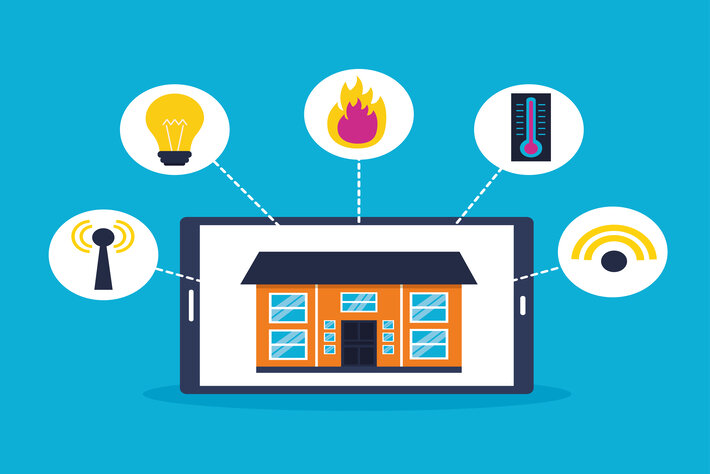
\includegraphics[width=1\linewidth]{Images/1.a.jpg}
    \caption{Smart Home System }
    \label{fig:enter-label}
\end{figure}

 